\subsection{GUI Tests}
Ich fange mit den GUI Tests an, die sich hauptsächlich auf den Editor beziehen. Die anderen Module teste ich in den Performance Tests. Im Vorgang werde ich Screenshots von Operationen auf Elementen zur Verfügung stellen, die alle Operationen im Editor auf dessen Elemente abdeckt.

\subsubsection{Input Control Tests}
In diesen Tests möchte ich die Funktionalität der implementierten Input Control bei input HTML-Elementen vom Typ Text auf die Probe stellen. Dies hat zum Ziel, dass meine Eingaben die minimalen und maximalen Werte für die input fields austesten und von der Anwendung Usereingaben automatisch korrigiert werden. Die Tests habe ich mit der Datei merged-sensoren-wissschreib.pdf mit 11 Seiten durchgeführt. Die Tabelle \ref{table:reader-input} beschreibt alle Test im Reader, \ref{table:creator-input} steht für Creator-Tests, \ref{table:splitter-input} verdeutlicht Splitter-Test, \ref{table:text-input} führt alle Texteditor eigenen Tests auf, \ref{table:draw-input} enthält Pencil Eraser Size Tests, \ref{table:shape-input} bildet Geometrieeditor-Tests ab, \ref{table:img-input} zeigt alle Bildeditor-Tests und alle im Editor mehrfach vorkommende wurden in \ref{table:editor-input} getestet. Wenn ich in eine Tabellenzelle invalid input schreibe, bedeutet das, dass die Eingabe stehen bleibt aber nicht ausgeführt wird. Die list of pages im Splitter funktioniert analog zu den Seitenlisten in den Auswählfiltern des Editors.

\begin{table}[!htbp]
	\centering
	\begin{tabular}{|p{4cm}|p{3cm}|p{3cm}|p{3cm}|}
		\hline
		\textbf{input field}				& \textbf{Input} 	& \textbf{Output-Korrektur}	\\ 
		\hline
		Page Counter						& hello 			& invalid input				\\
		Page Counter						& hello 1			& hello1 (invalid input)	\\
		Page Counter						& 0 				& 1							\\ 
		Page Counter						& 10 				& 9 						\\ 
		Page Counter						& 1.2 				& 1 						\\ 
		Zoom 								& 0					& 1\%  						\\
		Zoom 								& 801 \% 			& 800\% 					\\ 
		Zoom 								& 20 .1 			& 20\% 						\\ 
		Zoom 								& .2\% 				& 1\% 					\\ 
		Zoom 								& -.6 				& 1\% 						\\ 
		\hline
	\end{tabular}
	\caption{input field Tests im Reader}
	\label{table:reader-input}
\end{table}	

\begin{table}[!htbp]
	\centering
	\begin{tabular}{|p{4cm}|p{3cm}|p{3cm}|p{3cm}|}
		\hline
		\textbf{input field}		& \textbf{Input} 	& \textbf{Output-Korrektur}	\\ 
		\hline
		Number of Pages 			& 0 				& 1 						\\ 
		Number of Pages				& 5001 				& 5000  					\\ 
		Number of Pages				& 1.5 				& 1  						\\ 
		Width und Height			& 9 				& 10						\\  
		Width und Height			& 10001 			& 10000 					\\  
		Width und Height			& 21 0.6			& 210	 					\\
		\hline
	\end{tabular}
	\caption{input field Tests im Creator}
	\label{table:creator-input}
\end{table}

\begin{table}[!htbp]
	\centering
	\begin{tabular}{|p{4cm}|p{3cm}|p{3cm}|p{3cm}|}
		\hline
		\textbf{input field}	& \textbf{Input} 	& \textbf{Output-Korrektur}		\\ 
		\hline
		list of pages			& 1,2,11			& Eingabe gelöscht  			\\ 
		list of pages			& 1,2,2,5			& 1,2,5 						\\ 
		list of pages			& 1 0,2				& 2,10							\\ 
		\hline
	\end{tabular}
	\caption{input field Tests im Splitter}
	\label{table:splitter-input}
\end{table}

\begin{table}[!htbp]
	\centering
	\begin{tabular}{|p{4cm}|p{3cm}|p{3cm}|p{3cm}|}
		\hline
		\textbf{input field}			& \textbf{Input} 			& \textbf{Output-Korrektur}		\\ 
		\hline
		Line Height 					& 0 						& 1  							\\
		Line Height						& 30 1 						& 300 							\\ 
		Line Height						& 30.1 						& 30							\\ 
		Font Size 						& 2							& 3  							\\
		Font Size						& 501						& 500 							\\ 
		Font Size						& 60. 6 7					& 60 							\\ 
		\hline
	\end{tabular}
	\caption{input field Tests im Texteditor}
	\label{table:text-input}
\end{table}

\begin{table}[!htbp]
	\centering
	\begin{tabular}{|p{4cm}|p{3cm}|p{3cm}|p{3cm}|}
		\hline
		\textbf{input field}			& \textbf{Input} 			& \textbf{Output-Korrektur}		\\ 
		\hline
		Pencil Eraser Size 					& 0 .0001					& 0.1  						\\
		Pencil Eraser Size					& 4 0 1 					& 401						\\ 
		Pencil Eraser Size					& 501 						& 500						\\ 
		\hline
	\end{tabular}
	\caption{input field Tests im Zeichnen Editor}
	\label{table:draw-input}
\end{table}

\begin{table}[!htbp]
	\centering
	\begin{tabular}{|p{4cm}|p{3cm}|p{3cm}|p{3cm}|}
		\hline
		\textbf{input field}			& \textbf{Input} 			& \textbf{Output-Korrektur}	\\ 
		\hline
		Triangle Point 					& 0							& 1  						\\
		Triangle Point					& 30 01 					& 3000						\\ 
		Triangle Point					& 5.6 						& 5							\\ 
		Stroke Width 					& 00						& 0.1  						\\
		Stroke Width					& 1 00.1 					& 100						\\ 
		\hline
	\end{tabular}
	\caption{input field Tests im Shape Editor}
	\label{table:shape-input}
\end{table}

\begin{table}[!htbp]
	\centering
	\begin{tabular}{|p{4cm}|p{3cm}|p{3cm}|p{3cm}|}
		\hline
		\textbf{input field}		& \textbf{Input} 			& \textbf{Output-Korrektur}	\\ 
		\hline
		Opacity 					& 0.001						& 0.01  					\\
		Opacity						& -3 						& 0.01						\\ 
		Opacity						& 2 						& 1							\\ 
		\hline
	\end{tabular}
	\caption{input field Tests im Bildeditor}
	\label{table:img-input}
\end{table}

\begin{table}[!htbp]
	\centering
	\begin{tabular}{|p{4cm}|p{3cm}|p{3cm}|p{3cm}|}
		\hline
		\textbf{input field}	& \textbf{Input} 	& \textbf{Output-Korrektur}		\\ 
		\hline
		Rotate					& -361 						& -360  				\\
		Rotate					& 361 						& 360 					\\ 
		Rotate					& -30.3 					& -30  					\\
		Rotate					& 4 0.5 					& 40 					\\
		Rotate					& .3 						& 0 					\\ 
		Rotate					& -.3 						& 0 					\\ 
		Scale Factor			& 0.01						& 0.1 					\\
		Scale Factor			& 2 0 . 1					& 20 					\\
		Scale Factor			& .2						& 0.2 					\\
		Scale Factor			& 000.3						& 0.3 					\\
		Width und Height		& 0.1						& 1 					\\
		Width und Height		& 3000.02					& 3000 					\\
		Width und Height		& 100,2						& invalid input 		\\
		\hline
	\end{tabular}
	\caption{Test von mehrfach vorkommenden input fields im Editor}
	\label{table:editor-input}
\end{table}

\subsubsection{Editorergebnisse}
Bei diesen Tests werde ich Operationen auf verschiedene Editorelemente ausführen und zeigen wie sie ineinander greifen. Entsprechende Screenshots füge ich zur Dokumentation dazu. Alle Operationen wurden mit editor-ergebnisse-tests.pdf mit unterschiedlichen Seitengrößen ausgeführt. Abbildung \ref{fig:text-ops} zeigt ein Typografiedesign, \ref{fig:draw-ops} stellt eine freie Zeichnung dar, \ref{fig:shape-ops} bildet eine Geometriekomposition ab und \ref{fig:img-ops} visualisiert eine Photokollage.

\textbf{Textoperationen:}
\begin{itemize}
	\item Text: TH Köln mit Zeilenumbruch
	\item Line Height: 50
	\item Custom Font: Marborn.ttf
	\item Font Size: 80
	\item Font Color: RGBA(8, 84, 8, 0.75)
	\item Rotation: 90 Grad
\end{itemize}

\begin{figure}[!htbp]
	\centering
	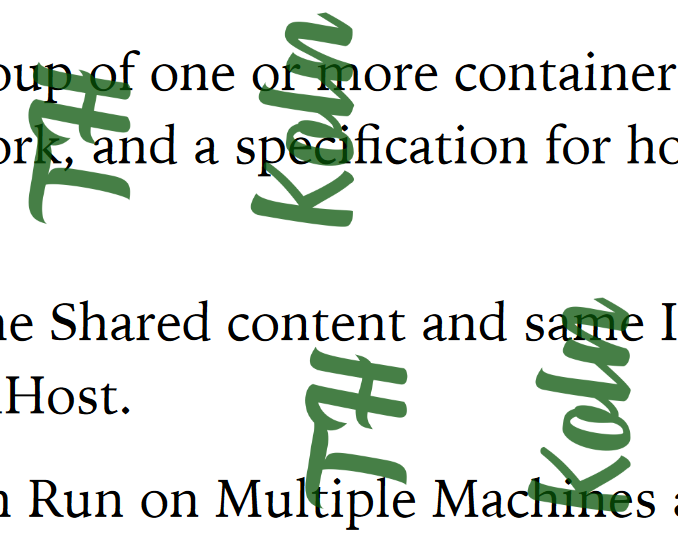
\includegraphics[width=0.6\textwidth]{"images/text-ops.png"}
	\caption{Typografiedesign}
	\label{fig:text-ops}
\end{figure}

\textbf{Zeichnen Operationen:}
\begin{itemize}
	\item Pencil Eraser Size: 10 (braune Linie)
	\item Pencil Color: RGBA(144, 81, 81, 0.9) (braune Linie)
	\item Pencil Eraser Size: 20 (blaue Linie)
	\item Pencil Color: RGBA(81, 143, 144, 1) (blaue Linie)
	\item Width Factor: 0.7 (Kopie)
	\item Height Factor: 1.5 (Kopie)
	\item Rotation: 45 Grad (Kopie)
\end{itemize}

\begin{figure}[!htbp]
	\centering
	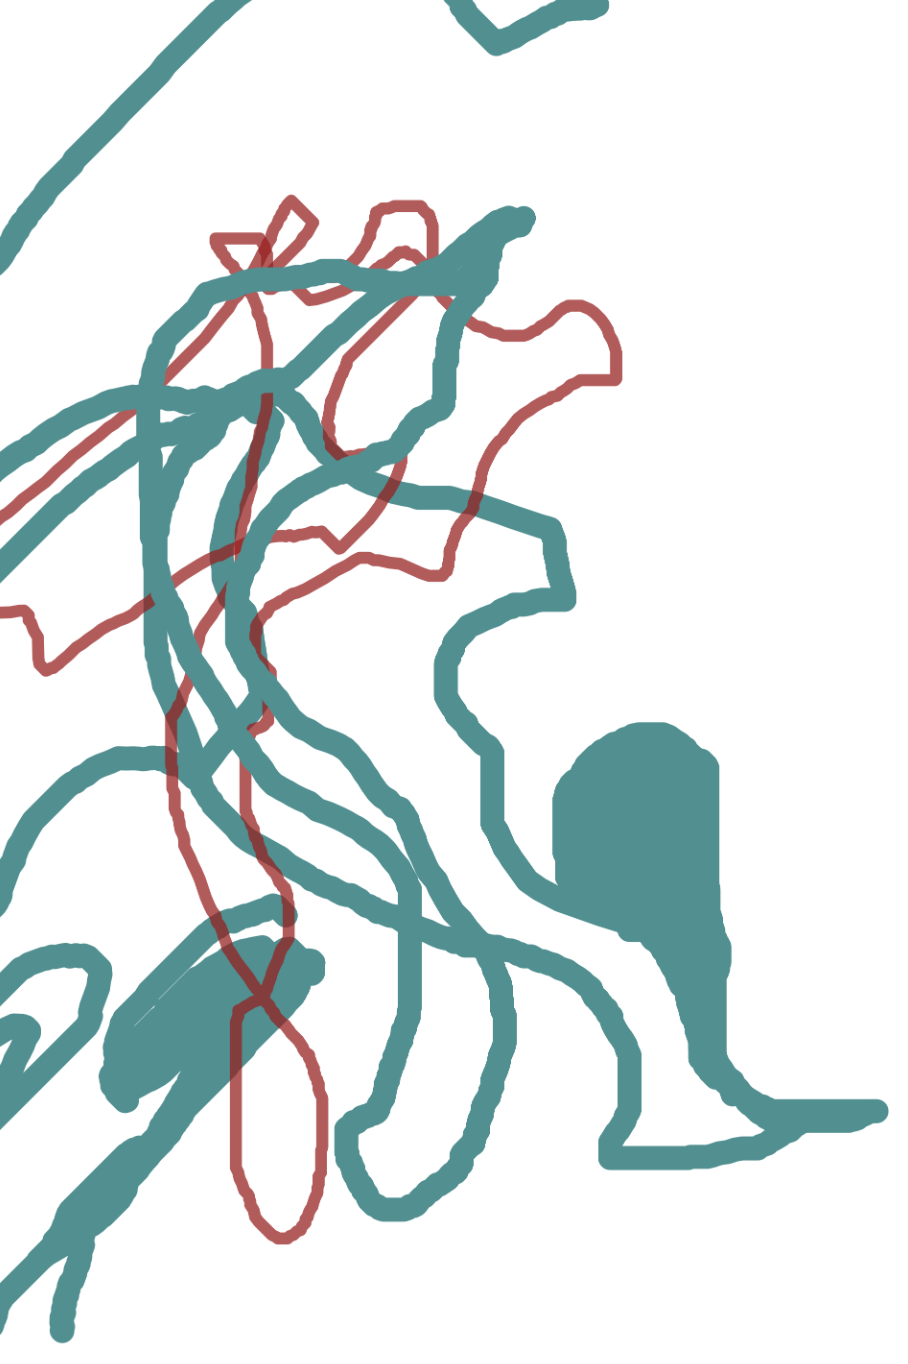
\includegraphics[width=0.7\textwidth]{"images/draw-ops.png"}
	\caption{Freie Zeichnung}
	\label{fig:draw-ops}
\end{figure}

\textbf{Geometrie Operationen:}
\begin{itemize}
	\item Point X: 50 (Dreieck)
	\item Point Y: 100 (Dreieck)
	\item Fill Color: RGBA(0, 0, 0, 0.67) (Dreieck)
	\item No Stroke (Dreieck)
	\item Rotation: 30 Grad (Kopie Dreieck)
	\item Stroke Color: RGBA(92, 7, 7, 1) (Ellipse) 
	\item Stroke Width: 9 (Ellipse)
	\item Fill Color: RGBA(181, 18, 18, 1) (Ellipse)
	\item Width: 200 (Ellipse)
	\item Height: 70 (Ellipse)
	\item Rotation: -30 (Ellipse)
	\item Scale Factor: 1.5 (Quadrat)
	\item Rotation: 45 Grad (Quadrat)
\end{itemize}

\begin{figure}[!htbp]
	\centering
	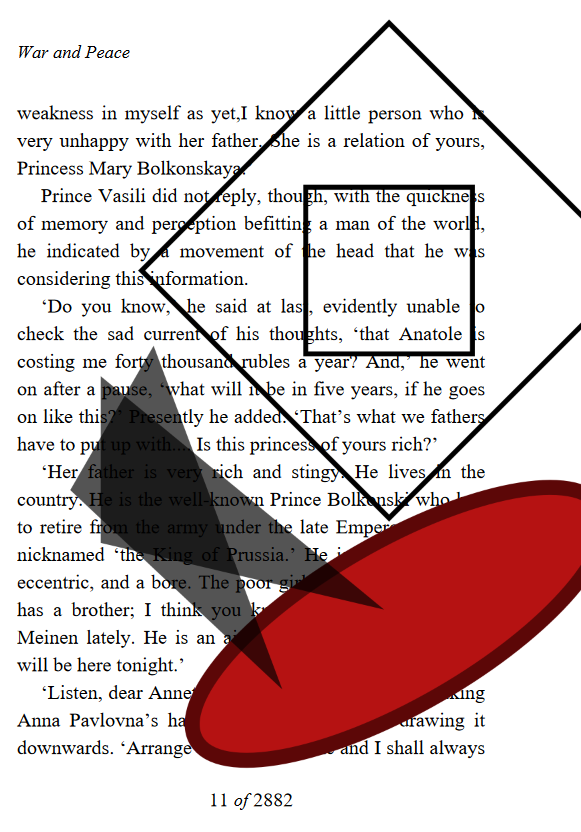
\includegraphics[width=0.7\textwidth]{"images/shape-ops.png"}
	\caption{Geometrieakomposition}
	\label{fig:shape-ops}
\end{figure}

\textbf{Bildoperationen:}
\begin{itemize}
	\item Opacity: 0.7 (Kopie Schmetterling)
	\item Width: 400 (Tiger)
	\item Height: 200 (Tiger)
	\item Rotation: 45 (Tiger)
	\item Scale Factor: 0.9 (Musikgerät)
\end{itemize}

\begin{figure}[!htbp]
	\centering
	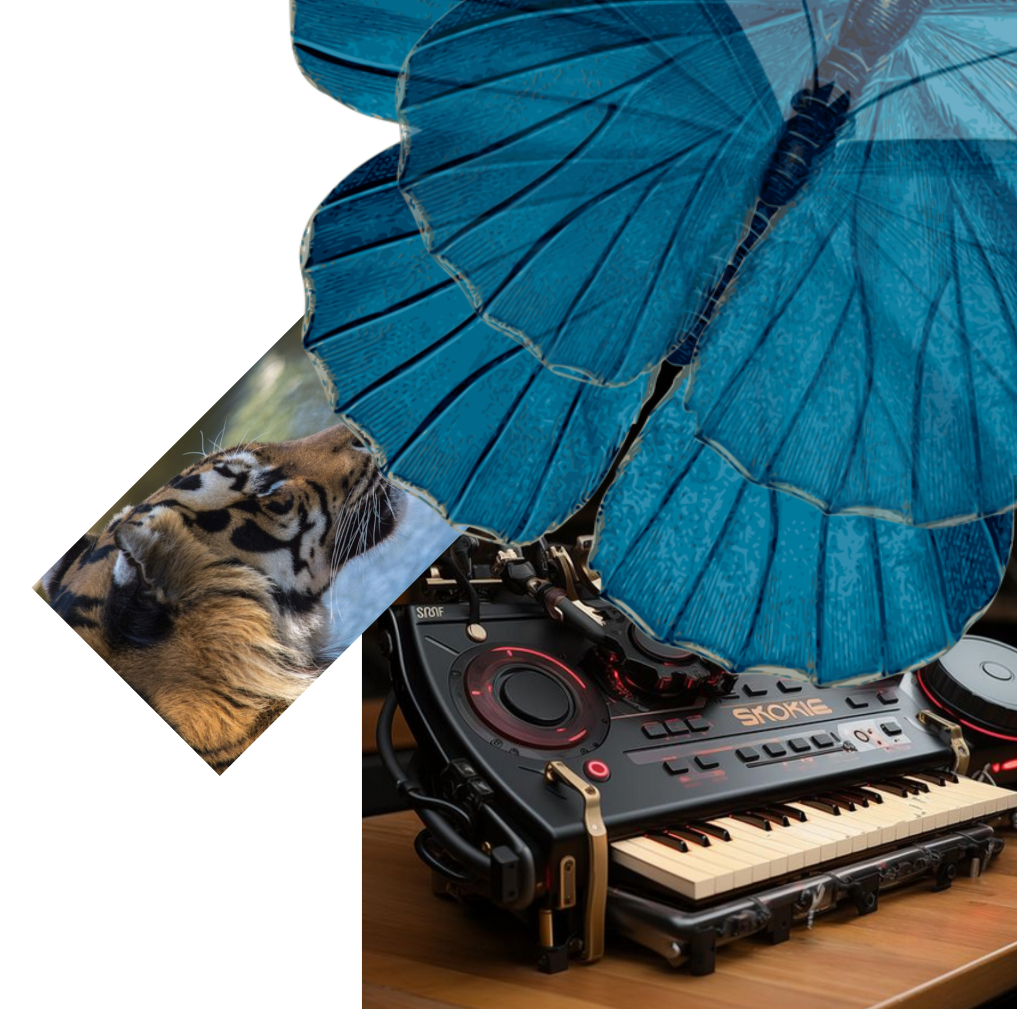
\includegraphics[width=0.9\textwidth]{"images/img-ops.png"}
	\caption{Fotokollage}
	\label{fig:img-ops}
\end{figure}